\begin{enigme}[Repas gastronomique]

\smallskip

  \begin{minipage}{8.5cm}
    28 personnes participent à un repas gastronomique. Le prix normal
    est de 26 \euro{} sauf pour les étudiants et les enfants. Ces
    derniers paient respectivement 17 \euro{} et 13 \euro. La somme
    totale recueillie est de 613 \euro.

    Calculer le nombre d'étudiants et d'enfants ayant participé au
    repas.

    Proposer trois méthodes dont une algorithmique pour résoudre ce
    problème.
  \end{minipage}\quad
\raisebox{-8mm}{\begin{minipage}{8cm}
  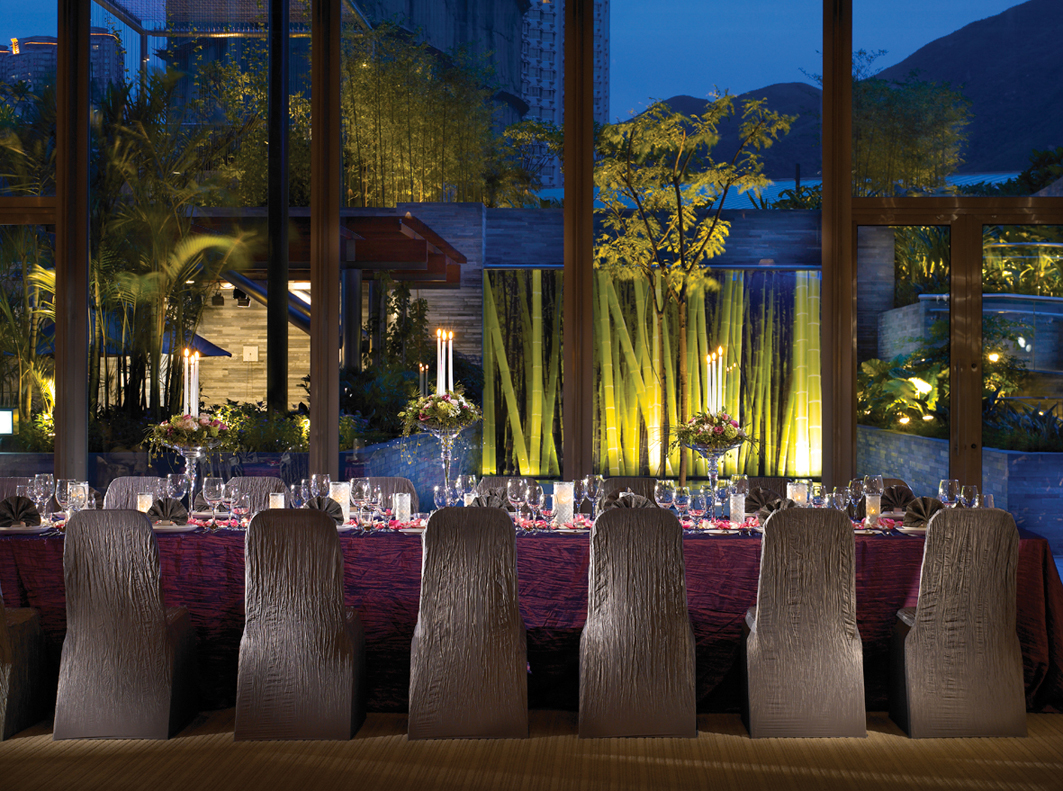
\includegraphics[width=.9\linewidth]{Novotel_Citygate_Hong-Kong-Banquet-Long_Table}
\end{minipage}}

\end{enigme}\vspace{0.5cm}

\begin{enigme}[Jour et mois de naissance]

% \begin{center}
% 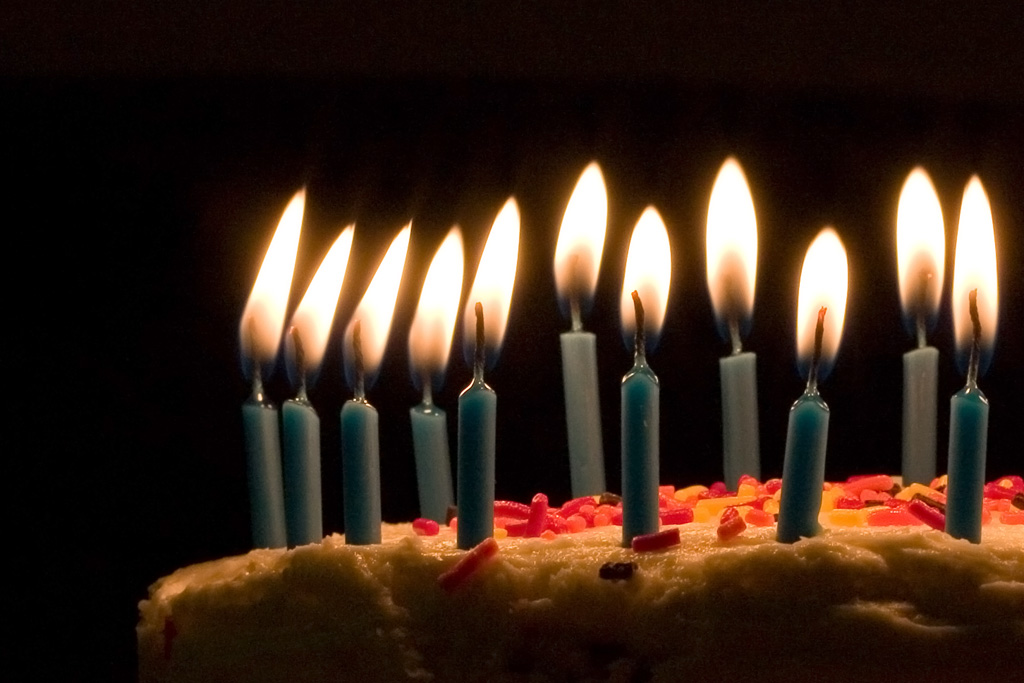
\includegraphics[width=5cm]{Blue_candles_on_birthday_cake}
% \end{center}\vspace{-5pt}

En multipliant mon jour de naissance par 12 et mon mois de naissance par 31, j'obtiens 442.

Quelle est ma date de naissance ? On proposera deux méthodes dont une algorithmique à ce problème. 

(On ne demande pas l'année, ouf !)
\end{enigme}\vspace{0.5cm}

\begin{enigme}[Théorème des restes chinois]

  Une bande de 17 pirates possède un trésor constitué de pièces d'or d'égale valeur. Ils projettent de se les partager de manière égale, et de donner le reste au cuisinier chinois. Celui-ci recevrait alors 3 pièces. Mais les pirates se querellent, et six d'entre eux sont tués. Un nouveau partage donnerait au cuisinier 4 pièces. Dans un naufrage ultérieur, seuls le trésor, six pirates et le cuisinier sont sauvés, et le partage donnerait alors 5 pièces d'or à ce dernier.

Quelle est la fortune minimale que peut espérer le cuisinier s'il décide d'empoisonner le reste des pirates ?\vspace{0.5cm}

% \parbox{0.28\textwidth}{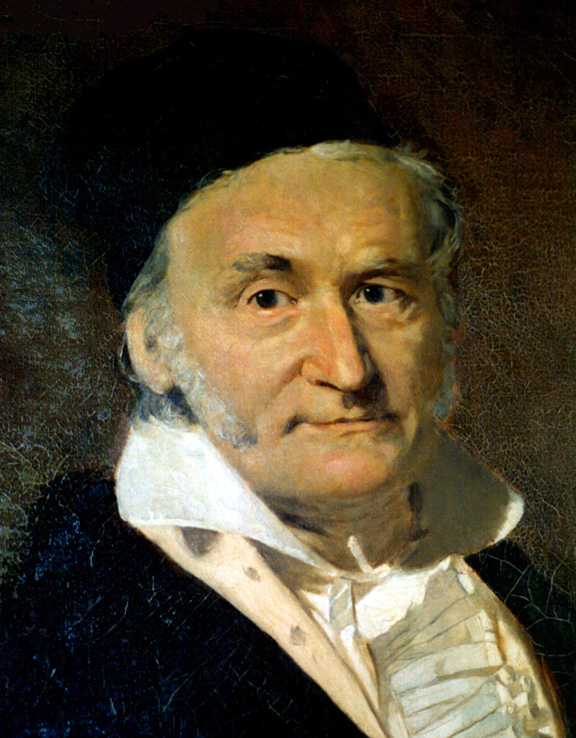
\includegraphics[width=0.25\textwidth]{Carl_Friedrich_Gauss}}
% \parbox{0.57\textwidth}{\begin{minipage}{0.6\textwidth}
% Le grand nom pour la résolution moderne de ce problème est évidemment celui de Carl Friedrich Gauss (1777-1855), à qui nous devons, bien au-delà de la solution complète du problème des congruences simultanées, la définition des congruences et leur constitution en une nouvelle arithmétique. Celle-ci donnera naissance à la théorie des corps finis et notamment à son application contemporaine au cryptage.
% \end{minipage}}
\end{enigme}